%!TEX root = ../../main.tex

\chapter{Einführungen}

\section{A-priori-Wahrscheinlichkeit}

Die A-priori-Wahrscheinlichkeit ist in den Naturwissenschaften der Wahrscheinlichkeitswert, der aufgrund von allgemeinem Vorwissen über die Eigenschaften des Systems
(ein Beispiel ist der Würfel, mit seinen symmetrischen Eigenschaften) gewonnen wird. Die A-priori-Wahrscheinlichkeiten sind die Grundvorraussetzungen
bei der Berechnung von bedingten Wahrscheinlichkeiten.
Die älteste Methode für die Bestimmung von A-priori-Wahrscheinlichkeiten stammt von Laplace. Sofern es keinen expliziten Grund gibt, die ursprünglich
offensichtliche Annahme zu ändern, wird allen Elementarereignissen die gleiche Wahrscheinlichkeit zugeordnet. (\cite[S. 80f]{Pap:1995})

Definiert man die Zufallsvariable $X$ als Ergebnis eines Würfelwurfes ergibt sich die folgende Wahrscheinlichkeitsverteilung:

\begin{multicols}{3}
    \begin{itemize}
        \item $P(X = 1) = \frac{1}{6}$
        \item $P(X = 2) = \frac{1}{6}$
        \item $P(X = 3) = \frac{1}{6}$
        \item $P(X = 4) = \frac{1}{6}$
        \item $P(X = 5) = \frac{1}{6}$
        \item $P(X = 6) = \frac{1}{6}$
    \end{itemize}
\end{multicols}

Dies ist allerdings nur der Fall, solange man keinen Grund hat anzunehmen, dass der Würfel manipuliert sei. Es handelt sich also um Elementarereignisse, der
alle dieselbe Wahrscheinlichkeit zugeordnet sind.

\section{Bedingte Wahrscheinlichkeit}

Die Wahrscheinlichkeit, dass das Ereignis $A$ eintritt, unter der Vorraussetzung, dass $B$ schon eingetreten ist, lässt sich mit

\begin{equation*}
    P(A | B) = \frac{P(A \cap B)}{P(A)}
\end{equation*}

berrechnen (\cite[404]{Papula:2014}).
\autoref{fig:bedingte-wahrscheinlichkeit} zeigt bedingte Wahrscheinlichkeiten im Kontext von Baumdiagrammen.

\begin{figure}
    \centering
    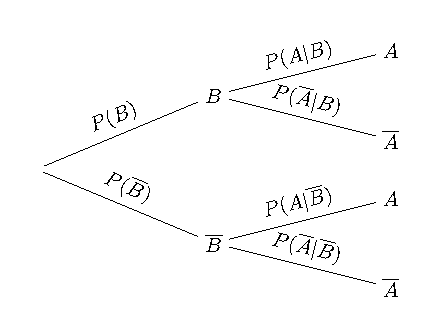
\includegraphics{tex/bedingte.pdf}
    \caption{Baumdiagram mit bedingten Wahrscheinlichkeiten}\label{fig:bedingte-wahrscheinlichkeit}
\end{figure}

\section{Satz von Bayes}

Der Satz von Bayes ist ein mathematischer Satz, der aus der Wahrscheinlichkeitstheorie stammt. Er beschreibt die Berechnung bedingter
Wahrscheinlichkeiten.
Der Satz ist nach dem englischen Mathematiker Thomas Bayes benannt und wird auch als Formel von Bayes oder als Bayes-Theorem bezeichnet. (\cite[S.406f]{Papula:2014})

\subsection{Formel}

Für zwei Ereignisse \textit{A} und \textit{B} mit \textit{P(B) > 0} lässt sich die Wahrscheinlichkeit von \textit{A} unter der Bedingung, dass \textit{B} eingetreten
ist, durch die Wahrscheinlichkeit von \textit{B} unter der Bedingung, dass \textit{A} eingetreten ist, errechnen:

\begin{equation*}
    P(A | B) = \frac{P(B | A) \cdot P(A)}{P(B)}
\end{equation*}

Hierbei ist

\begin{itemize}
    \item $P(A | B)$ die bedingte Wahrscheinlichkeit von $A$ unter der Bedingung $B$,
    \item $P(B | A)$ die bedingte Wahrscheinlichkeit von $B$ unter der Bedingung $A$,
    \item $P(A)$ die A-priori-Wahrscheinlichkeit von $A$ und
    \item $P(B)$ die A-priori-Wahrscheinlichkeit von $B$.
\end{itemize}

Bei endlich vielen Ereignissen lautet der Satz von Bayes:

Wenn $A_i, i = 1,..., N$ eine Zerlegung der Ergebnismenge in disjunkte Ereignisse ist, gilt für die bedingte Wahrscheinlichkeit $P(A_i | B)$

\begin{equation} \label{equ:bayes}
    P(A_i | B) = \frac{P(B | A_i) \cdot P(A_i)}{P(B)} \underbrace{= \frac{P(B | A_i) \cdot P(A_i)}{\sum_{j = 1}^{N} P(B | A_j) \cdot P(A_j)}}_{Marginalisierung}
\end{equation}

(\cite[S.406f]{Papula:2014})

Bei den Betrachtungen des Monty-Hall-Problems sind die A-priori-Wahrscheinlichkeiten $P(A_1) = P(A_2) = ... = P(A_N) = P(A)$ alle gleich. Dadurch lässt sich \autoref{equ:bayes} vereinfachen:

\begin{equation} \label{equ:bayes_simpl}
    P(A_i | B)  = \frac{P(B | A_i) \cdot P(A)}{\sum_{j=1}^{N} P(B | A_j) \cdot P(A)}  = \frac{P(B|A_i)}{\sum_{j=1}^{N} P(B | A_j)}
\end{equation}
